% ltex: language=it
\chapter{Ciclo di Vita di un Progetto Informatico}\label{chap:ciclo_di_vita_di_un_progetto_informatico} % (fold)
Il \textbf{ciclo di vita dei progetti} approvati in fase di pianificazione è riportato di seguito.
È inoltre fornito il dettaglio delle principali tematiche affrontate in ogni fase.
\begin{cimage}
    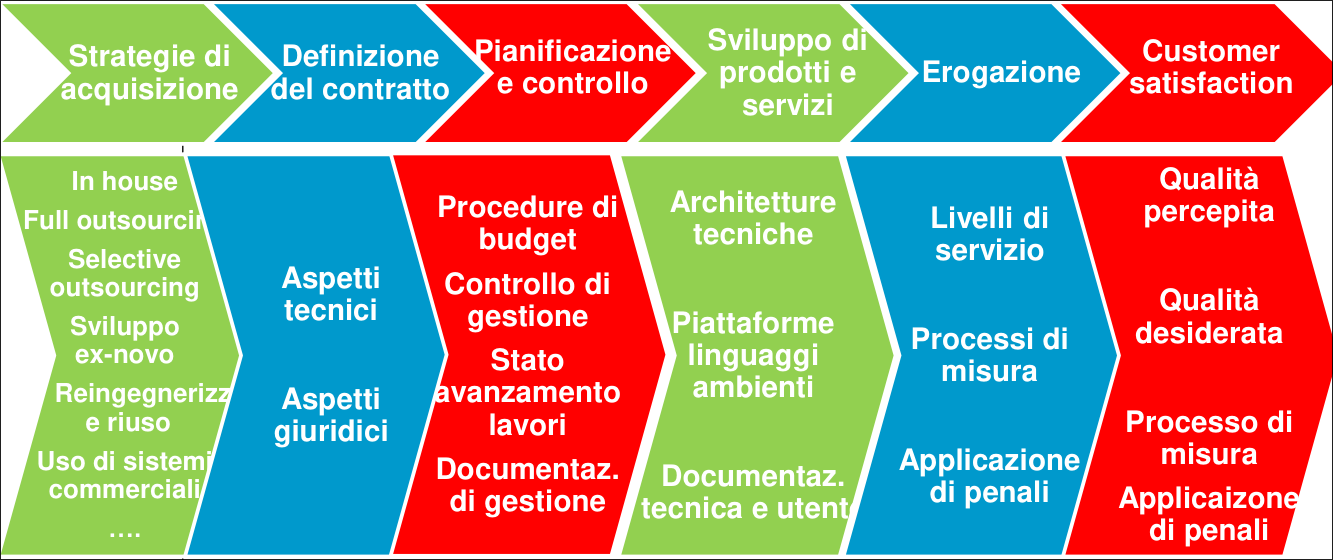
\includegraphics[width=.8\textwidth]{assets/ciclo-vita-prog-fasi-visual.png}
\end{cimage}
%
\section{Strategie di Acquisizione: Make or Buy?}\label{sec:cv_strategie_di_acquisizione_make_or_buy} % (fold)
La realtà è molto complessa, per commentarla è utile schematizzare, ma con spirito critico:
\begin{itemize}
    \item quasi nessuno fa tutto in casa;
    \item l'affidamento totale all'esterno è raro, e se estremo e non governato diventa pericoloso e potenzialmente inefficace;
\end{itemize}
È necessario distinguere i seguenti termini:
\begin{itemize}
    \item \textbf{acquisto sul mercato di un bene o servizio}: accezione generica riferita alla scelta di acquisizione da terzi (Buy) invece che realizzare internamente (Make) un bene o un servizio;
    \item \textbf{esternalizzazione (\hyperref[sub:ftt_outsourcing]{outsourcing})}: presuppone una qualche forma di stabilità del rapporto di ``collaborazione'' tra l'impresa e il terzista con una prospettiva di medio termine;
\end{itemize}
%
\subsection{Outsourcing: Classificazione}\label{sub:cv_outsourcing_classificazione} % (fold)
\begin{description}
    \item[In base alla missione affidata al Fornitore] Esistono i tipi: \red{\ac{ito}}, \red{Business Process Outsourcing}
        \begin{definition}{Information Technology Outsourciung}{ito}
            L'outsourcing delle attività di sviluppo, esercizio, manutenzione dei \hyperref[sub:il_sistema_informativo]{Sistemi Informativi} e delle risorse informatiche.
            \\
            Può essere:
            \begin{itemize}
                \item Full Outsourcing;
                \item Selective Outsourcing (spesso ``Multisourcing'');
            \end{itemize}
        \end{definition}
        \begin{definition}{Business Process Outsourcing}{bpo}
            Il \textbf{\ac{bpo}} è l'outsourcing dei processi operativi dell'organizzazione, di solito ``strumentali'' e non ``core'':
            \begin{multicols}{2}
                \begin{itemize}
                    \item personale;
                    \item contabilità e finanza;
                    \item assistenza agli utenti;
                    \item relazioni con gli utenti;
                    \item acquisti e forniture;
                    \item commercio elettronico su internet;
                \end{itemize}
            \end{multicols}
            \begin{note}
                Alcuni casi di servizi ``core'', con rapporti stretti di partnership fra \textbf{amministrazione} e \textbf{fornitore}
            \end{note}
        \end{definition}
    \item[In base all'ampiezza del mandato conferito al Fornitore] Esistono i tipi: \red{Full Outsourcing}, \red{Selective Outsourcing}
        \begin{definition}{Insourcing}{}
            La funzione IT è delegata a una società di servizi separata dall'organizzazione a cui fornisce servizi ma da essa posseduta, oppure è comunque formalizzato o quasi il rapporto fra struttura IT e altre strutture.
            \begin{quote}
                Fornisce e implementa nuovi servizi e architetture IT sulla base di \textbf{contratti informali} (controllo di gestione come centro di ricavi) o \textbf{contratti di servizio} (definizione di tariffe per i servizi);
            \end{quote}
            Nel caso di \hyperref[def:bpo]{\ac{bpo}} si parla di \textbf{Captive Company}: società ``prigioniera'' cioè fondata da un altra azienda con lo scopo di eseguire operazioni per conto dell'azienda madre;
        \end{definition}
        \begin{definition}{Selective Outsourcing}{}
            Nel \textbf{Selective Outsourcing} è \textbf{delegata a più fornitori esterni}: fornisce e implementa nuovi servizi e architetture IT sulla base di più contatti di durata limitata (circa 3-5 anni).
            \begin{note}
                L'organizzazione attua un approccio tattico per creare un ambiente competitivo: complessità gestionale accresciuta
            \end{note}
            \begin{description}
                \item[Pro]
                    \begin{multicols}{2}
                        \begin{itemize}
                            \item Clima di competizione fra i fornitori: riduzione costi e ottimizzazione della scelta;
                            \item Controllo del committente  su coordinamento e integrazione;
                            \item Riduzione dei singoli tempi di acquisizione;
                            \item Possibile semplificazione della gestione dei singoli contratti;
                            \item Minore rischio di insuccesso globale;
                        \end{itemize}
                    \end{multicols}
                \item[Contro]
                    \begin{itemize}
                        \item Aumento della complessità di gestione dei molti contratti;
                        \item Possibile ``scarica barile'';
                        \item Difficoltà di integrazione;
                    \end{itemize}
            \end{description}
        \end{definition}
        \begin{definition}{Full Outsourcing}{full-outsourcing}
            Nel \textbf{Full Outsourcing} la funzione IT è \textbf{delegata a un unico fornitore esterno} che fornisce e implementa nuovi servizi e architetture IT sulla base di un unico contratto di servizio.
            \emptyln{}
            L'organizzazione intende creare una partnership strategica con l'outsourcer: è il modello classico di \hyperref[sub:ftt_outsourcing]{outsourcing}, dove il contratto copre la maggior parte delle esigenze IT dell'organizzazione e ha una lunga durata, 5-10 anni.
            \begin{warning}
                Nella realtà è spesso una via di mezzo: non si ha un ``full'' outsourcing in quanto sono coinvolti più servizi in un'unica collaborazione
            \end{warning}
            \begin{description}
                \item[Pro] 
                    \begin{itemize}
                        \item Interfaccia unica;
                        \item Unitarietà e integrazione delle componenti;
                        \item Riduzione di costi e tempi di acquisizione;
                        \item Possibile semplificazione nella gestione del contratto (uno solo);
                    \end{itemize}
                \item[Contro] 
                    \begin{multicols}{2}
                        \begin{itemize}
                            \item Limitata ``ottimizzazione'' nella scelta;
                            \item Perdita di controllo;
                            \item Riduzione del potere negoziabile e lock-in;
                            \item Demotivazione del personale IT interno;
                            \item Rischio di insuccesso globale;
                            \item Complessità del singolo contratto;
                        \end{itemize}
                    \end{multicols}
            \end{description}
        \end{definition}
        \begin{definition}{Joint Venture}{}
            La funzione IT è \textbf{delegata a una società di servizi separata e indipendente} dall'organizzazione a cui fornisce sevizi in partecipazione con un fornitore: fornisce e implementa nuovi servizi de architetture IT sulla base di un contratto di servizio.
            \emptyln{}
            La maggioranza delle quote può essere dell'uno o dell'altro, a seconda che si voglia privilegiare il controllo del committente o la responsabilità e l'impegno del fornitore.
        \end{definition}
        \begin{note}[Consorzi e RTI]
            La funzione IT è delegata a un consorzio, stabile o temporaneo, costituito da più fornitori esterni: fornisce e implementa nuovi servizi e architetture IT sulla base di un unico contratto di servizio.
            L'organizzazione intende creare una partnership strategica con il Consorzio.
            \emptyln{}
            La complessità gestionale è superiore a quella del \hyperref[def:full-outsourcing]{Full Outsourcing}: difficoltà di omogeneizzazione delle diverse culture, conoscenze e sistemi.
            Spesso si tratta di un \textbf{RTI} (ovvero un raggruppamento temporaneo di imprese), cioè di una struttura costituita per l'occasione e non permanente.
        \end{note}
\end{description}
% subsection Outsourcing: Classificazione (end)
%
\subsection{Compiti e Responsabilità della Funzione IT}\label{sub:cv_compiti_e_responsabilit_della_funzione_it} % (fold)
\begin{note}[Compiti]
    \begin{itemize}
        \item \textbf{Progettazione}:
            \begin{itemize}
                \item studi di fattibilità e rappresentazione dei requisiti;
                \item stima investimenti e analisi dei costi/benefici;
                \item contratti e atti di gara;
            \end{itemize}
        \item \textbf{Pianificazione e Controllo}:
            \begin{itemize}
                \item pianificazione informatica coerente alla missione;
                \item definizione delle priorità dei progetti;
                \item verifica del raggiungimento degli obiettivi;
            \end{itemize}
        \item \textbf{Relazione con gli Utenti}:
            \begin{itemize}
                \item acquisizione dei requisiti e dei bisogni reali;
                \item verifica della soddisfazione degli utenti;
            \end{itemize}
        \item \textbf{Osservatorio sul mercato dell'IT}:
            \begin{itemize}
                \item controllo delle soluzioni proposte dal Fornitore;
                \item contenimento del rischio di perdita di controllo;
            \end{itemize}
    \end{itemize}
\end{note}
\begin{note}[Responsabilità]
    \begin{itemize}
        \item \textbf{Gestione dei Progetti (\red{Project Management})}:
            \begin{multicols}{2}
                \begin{itemize}
                    \item gestione dei rapporti con il Fornitore;
                    \item budget e controllo di gestione;
                    \item verifica lo stato di avanzamento dei lavori;
                    \item accettazione/collaudo dei prodotti;
                    \item misura dei livelli di servizio;
                    \item segnalazione tempestiva di rilievi e non conformità;
                    \item proposta di azioni correttive o preventive;
                    \item monitoraggio;
                \end{itemize}
            \end{multicols}
        \item \textbf{Gestione delle banche dati (Data Administration \& Data Architect)}: sorvegliare la qualità dei dati;
        \item \textbf{Gestione della sicurezza (Security Management)}:
            \begin{itemize}
                \item sorvegliare l'applicazione delle politiche di sicurezza;
                \item verificare il rispetto della normativa vigente;
            \end{itemize}
    \end{itemize}
\end{note}
% subsection Compiti e Responsabilità della Funzione IT (end)
%
\subsection{Fattori Chiave di Successo}\label{sub:cv_fattori_chiave_di_successo} % (fold)
\begin{itemize}
    \item \textbf{Scelta della strategia di Sourcing}:
        \begin{itemize}
            \item approccio progressivo;
            \item adattarsi al mutare di condizioni interne o esterne;
        \end{itemize}
    \item \textbf{Selezione del Fornitore}: ricerca delle garanzie necessarie a contenere i rischi;
    \item \textbf{Definizione del Contratto}:
        \begin{itemize}
            \item responsabilità reciproche Cliente-Fornitore;
            \item modelli di applicazione delle tariffe;
            \item pariteticità, correttezza, funzionalità, flessibilità;
        \end{itemize}
    \item \textbf{Governo del Contratto}
\end{itemize}
% subsection Fattori Chiave di Successo (end)
% section Strategie di Acquisizione: Make or Buy? (end)
%
\section{Strategie di Realizzazione}\label{sec:cv_strategie_di_realizzazione} % (fold)
Le necessità informatiche portano alla necessità di realizzare un software applicativo sono:
\begin{itemize}
    \item nuove esigenze di automazione di processi non coperti dal sistema informatico;
    \item adeguamento di applicazioni esistenti: \textbf{MAC} (Manutenzione Correttiva) e \textbf{MEV} (Manutenzione Evolutiva);
\end{itemize}
Le nuove esigenze di automazione possono essere risolte con modalità diverse:
\begin{description}
    \item[Sviluppo di programmi ad hoc] Utile quando le funzioni da informatizzare sono peculiari della specifica azienda o dove i sistemi commerciali esistenti richiedessero un notevole sforzo di adeguamento/integrazione.
        Maggiore possibilità di personalizzazione e maggiore incertezza sui tempi e costi di realizzazione; inoltre richiede competenze interne ed esterne specifiche;
    \item[Riuso di programmi ad hoc sviluppati per altre PA] Le pubbliche amministrazioni sono obbligate a condividere con altre le applicazioni sviluppate.
        \\
        Utile quando le funzioni da informatizzare sono simili a quelle già realizzate.
        Forti impatti sul \red{modello di business} delle \textit{software house} produttrici del software che dovranno orientarsi al mercato delle personalizzazioni.
    \item[Utilizzo di sistemi informatici open source] Questa soluzione ha un basso costo iniziale, un maggior controllo sul costo complessivo d'esercizio (\hyperref[sub:ftt_total_cost_ownership]{\ac{tco}}) e una maggiore indipendenza dai fornitori.
        \begin{note}
            Può determinare una maggiore trasparenza della soluzione grazie all'accesso ai sorgenti
        \end{note}
        \begin{warning}
            Maggiore \red{possibilità di personalizzazione}, tuttavia:
            \begin{multicols}{2}
                \begin{itemize}
                    \item ridotta compatibilità con standard commerciali quando questi rappresentano lo <<standard de facto>>;
                    \item supporto non sempre disponibile;
                    \item instabilità di mercato;
                    \item potenziale mancanza di una evoluzione del sistema nel tempo;
                \end{itemize}
            \end{multicols}
        \end{warning}
    \item[Utilizzo di sistemi informatici proprietari con ricorso a licenza d'uso] Rispetto al \textbf{software open source} fornisce normalmente una maggiore garanzia in termini di affidabilità e performance.
        Può essere necessario per compatibilità con altre soluzioni già presenti in azienda.
        Rispetto a soluzioni open source va comunque valutato il reale \hyperref[sub:ftt_total_cost_ownership]{\ac{tco}} anche considerando i rischi legati a mancanza di supporto adeguato, manutenzione correttiva ed evolutiva.
\end{description}
% section Strategie di Realizzazione (end)
%
\section{Definizione del Contratto}\label{sec:cv_definizione_del_contratto} % (fold)
\begin{definition}{Contratto}{}
    Il \textbf{contratto}, secondo l'art. 1321 del Codice Civile, è un accordo di due o più parti per costruire, regolare o estinguere tra loro un rapporto giuridico patrimoniale.
\end{definition}
Esistono diversi tipi di contratto:
\begin{description}
    \item[Contratto d'Appalto art. 1655 C.C.] L'appalto è il contratto con il quale una parte assume, con organizzazione dei mezzi necessari e con gestione a proprio rischio, il compimento di un'opera o di un servizio verso un corrispettivo in denaro
    \item[Contratto d'Opera art. 2222 C.C.] Prestazione di lavoro personale dell'obbligato
    \item[Contratto di Compravendita art. 1472 C.C.] Cessione/acquisizione di qualcosa
\end{description}
\begin{note}[Visione Manageriale]
    Un contratto ha l'obiettivo di \textbf{soddisfare} entrambe le parti, ed eventuali terzi interessati; se i risultati non vengono raggiunti, entrambi hanno fallito.
    Quindi un contratto deve:
    \begin{itemize}
        \item \textbf{definire}, in modo cooperativo tra le parti, \textbf{le prestazioni} in termini di contenuti, costi, qualità e responsabilità;
        \item \textbf{eliminare le ambiguità} nel rapporto tra le parti e prevenire difficoltà e situazioni anomale;
    \end{itemize}
    \begin{warning}
        Ma non può pretendere di \textbf{prevedere tutto} in dettaglio, quindi deve specificare non solo \textbf{obblighi} e \textbf{impegni} ma anche \textbf{procedure} e \textbf{regole di relazione}
    \end{warning}
\end{note}
%
\subsection{Gestione dei Contratti}\label{sub:cv_gestione_dei_contratti} % (fold)
Il successo di un contratto dipende da molti fattori fra cui:
\begin{itemize}
    \item competenze tecniche e legislative dei suoi estensori;
    \item competenze tecniche e manageriali del personale preposto al suo governo durante tutto il ciclo di vita;
\end{itemize}
Il contratto rappresenta il \textbf{principale strumento} a disposizione delle parti per evitare le ambiguità nel loro rapporto.
Un contratto ben strutturato facilità le attività degli organi preposti al governo del contratto stesso:
\begin{tasks}(2)    
    \task comitato guida;
    \task direzione dei lavori;
    \task monitoraggio;
    \task collaudo;
    \task certificazioni di qualità;
\end{tasks}
\begin{note}[Soggetti coinvolti nelle Attività Contrattuali]
    Per il committente:
    \begin{itemize}
        \item dirigenti implicati nella definizione delle scelte strategiche;
        \item personale della funzione acquisti;
        \item personale della funzione legate;
        \item personale della funzione sistemi informativi;
        \item personale utente dei sistemi informativi;
    \end{itemize}
    Per il fornitore:
    \begin{itemize}
        \item dirigenti implicati nella definizione delle offerte;
        \item personale della funzione commerciale;
        \item personale della funzione legale;
        \item personale della funzione che eroga i servizi ICT;
        \item personale della funzione di assicurazione qualità;
    \end{itemize}
\end{note}
% subsection Gestione dei Contratti (end)
%
\subsection{Struttura di un Contratto}\label{sub:cv_struttura_di_un_contratto} % (fold)
Un contratto è diviso in due parti:
\begin{itemize}
    \item \textbf{Parte Nominativa}: il corpo del contratto;
    \item \textbf{Parte Operativa}: \red{Capitolato Tecnico} e \red{Offerta};
\end{itemize}
\begin{description}
    \item[Corpo del Contratto] Definisce e correla:
        \begin{itemize}
            \item aspetti tecnici, con la definizione dei beni e servizi oggetto del contratto;
            \item modalità, tempi e condizioni;
            \item relazioni fra cliente e fornitore;
            \item corrispettivi (pagamenti);
        \end{itemize}
    \item[Capitolato Tecnico] Predisposto dal cliente insieme al bando in caso di gara: recepisce le indicazioni dello \hyperref[chap:studio_di_fattibilita]{studio di fattibilità}.
        Fornisce al fornitore le informazioni di dettaglio utili per preparare l'offerta, di solito anche l'indice dell'offerta stessa.
        \begin{note}
            Allegato tecnico al corpo del contratto assieme all'offerta del fornitore
        \end{note}
    \item[Offerta Tecnica] Redatta dal fornitore in risposta a quanto richiesto dal cliente nel \red{Capitolato Tecnico}: corrisponde ai criteri di valutazione indicati nel bando di gara e/o nella lettera di invito.
        Ha lo scopo di dimostrare al cliente la capacità del fornitore di soddisfare quanto richiesto nel \textbf{Capitolato Tecnico} indicando ``come''.
        \\
        Possibili allegati:
        \begin{itemize}
            \item piano di progetto;
            \item piano della qualità;
        \end{itemize}
\end{description}
\begin{warning}[Spesso ci sono sovrapposizioni fra le varie parti, con anche incoerenze]
    In caso di gara, corpo e capitolato fanno parte della documentazione predisposta dal committente, mentre l'offerta è la ``risposta'' del fornitore.
    \emptyln{}
    Difficile descrivere in modo tassonomico la struttura di un contratto che varia fortemente in base al suo oggetto, \textit{procederemo per esempi} con un contratto di grandi dimensioni in ambito delle Pubbliche Amministrazioni.
\end{warning}
% subsection Struttura di un Contratto (end)
% section Definizione del Contratto (end)
% chapter Ciclo di Vita di un Progetto Informatico (end)
